\section{Einleitung und Versuchsziel}
\label{sec:aufgabenstellung}
Die Destillation und Rektifikation von Stoffgemischen ist ein essentielles Trennverfahren in der chemischen Industrie. Um Berechnungen dazu ausführen zu können, muss das Dampf-Flüssig-Gleichgewicht bekannt sein. Eben diese Abhängigkeiten zwischen Temperatur, Druck und den Zusammensetzungen der flüssigen und der Dampfphase soll im Laborversuch, anhand eines binären Gemisches aus Ethanol und Cyclohexan, untersucht werden. Aus den gewonnenen Daten werden das Siede-/Taudiagramm, das Gleichgewichtsdiagramm, die Partialdrücke und die Aktivitätskoeffizienten abgeleitet. 

\section{Theoretische Grundlagen}

\subsection{Der Azeotrope Punkt}
Ein Azeotrop ist ein Gemisch aus mindestens zwei Komponenten in einem bestimmten Mischungsverhältnis. Die Besonderheit ist, dass sich dieses Gemisch wie ein Reinstoff verhält. Es lässt sich nicht ohne weiteres Destillieren um die Komponenten zu trennen.
\subsection{Refraktometrie}
\subsubsection*{Das Abbe-Refraktometer}
Das Abbe-Refraktometer ist ein Messgerät zur Bestimmung des Brechungsindexes einer Flüssigkeit. Es ist nach seinem Erfinder Ernst Abbe benannt. Der schematische Aufbau ist in Abb. \ref{fig:refraktometer} dargestellt. Es sind gut die beiden Prismen P1 und P2 zu sehen, zwischen welchen sich der Probenfilm befindet. Das Licht wird gebrochen, sodass ein Horizont entsteht. Auf der einen Seite ist Licht und auf der anderen Seite nicht. Je nach Zusammensetzung der Probe wird das Licht in einem anderen Winkel gebrochen. Dieser Horizont wird an einem Fadenkreuz ausgerichtet. Das Instrument ist so kalibriert, dass die beim Einstellen des Horizontes auf das Fadenkreuz mitbewegte Skala, den Brechungsindex anzeigt. 
Weil der Brechungsindex auch stark von der Temperatur beeinflusst wird ist das Refraktometer mit einem Thermostaten verbunden.

\begin{figure}[h!]
	\centering
	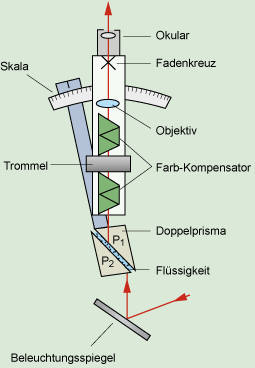
\includegraphics[width=0.7\linewidth]{img/refraktometer}
	\caption{Funktionsprinzip eines Abbe-Refraktometers \cite{refraktometer}}
	\label{fig:refraktometer}
\end{figure}

\subsubsection*{Die Na-D-Linie}

Die Messung des Brechungsindexes erfolgt bei einer spezifischen Wellenlänge, da diese Einfluss auf den Reflexionswinkel hat. Üblich ist dabei die Verwendung der  Wellenlänge  \SI{589}{\nano\meter}. Diese entspricht einer spezifischen Wellenlänge im Spektrum des Natriums und kann mit einer Natriumdampflampe erzeugt werden. Bei modernen Refraktometern wird sie durch einen optischen Filter aus dem kontinuierlichen Spektrum einer Glühlampe extrahiert.
\FloatBarrier
\subsection{Die Gibbs'sche Phasenregel}
Anhand der Gibbs'schen Phasenregel lassen sich die Freiheitsgrade eines Systems berechnen. Die Formel ist in Gleichung \eqref{gl:gibbs} dargestellt. F steht für die Anzahl der Freiheitsgrade, N für die Anzahl der Komponenten und P für die Anzahl an Phasen.
\vspace{-2mm}
\begin{equation}\label{gl:gibbs}
F=N-P+2
\end{equation}
\subsubsection*{Anzahl der Freiheitsgrade}
Für das betrachtete System kann nun in die Gibbs'sche Phasenregel eingesetzt werden. Es gibt die Stoffe Ethanol und Cyclohexan. Wir betrachten außerdem ein Zweiphasensystem, mit der flüssigen und gasförmigen Phase. Daraus ergeben sich zwei Freiheitsgrade (vgl. \eqref{gl:bspGibbs}). In der Fachsprache kommt dafür die Bezeichnung "`bivariant"' zum Einsatz.

\begin{flalign}\label{gl:bspGibbs}
	F&=2-2+2\\
	&=\underline{2}
\end{flalign}
\subsubsection*{Variablen des Systems}

In Anbetracht der Tatsache dass das System offen gegen die Atmosphäre ist, kann es als isobar angenommen werden. Über die Zusammensetzung der flüssigen Phase kann frei verfügt werden. Die Temperatur stellt sich dementsprechend nach einiger Zeit von selbst ein. 
\subsection{Raoult-Dalton'sches-Gesetz}
Das Raoult-Dalton'sche-Gesetz ist aus dem Raoult'schen und dem Dalton'schen Gesetz zusammengesetzt. Es beschreibt den Zusammenhang zwischen der Temperatur, dem Druck, den Partialdrücken und der Zusammensetzung von Flüssigkeit und Dampf eines Systems. Zur Beschreibung realer Mischungen bei niedrigen Drücken muss der Aktivitätskoeffizient mit einbezogen werden. Der fertige Zusammenhang ist in Gleichung \eqref{gl:raudalt} vermerkt.
\begin{equation}\label{gl:raudalt}
	p_i=x_i^V*p=x_i^L*p_i^0(T)*\gamma_i
\end{equation}
\subsection{Antoine-Gleichung}
Als Modell zur Beschreibung des Sättigungsdampfdruckes in Abhängigkeit von der Temperatur, wird die Antoine-Gleichung \eqref{gl:anton} genutzt. Diese basiert auf der Clapeyron-Gleichung \eqref{gl:clapeyron}. Sie ist aber besser zur Beschreibung realer Systeme geeignet, da in ihr ein dritter Stoffparameter C einbezogen wird. Die Antoine-Parameter A,B und C sind für viele Systeme bereits tabelliert. Dabei ist stets auf den temperaturabhängigen Geltungsbereich zu achten.
\begin{equation}\label{gl:clapeyron}
ln(p^\circ)=A-\frac{B}{T}
\end{equation}
\begin{flalign}\label{gl:anton}
\lg(p)=A-\frac{B}{C+\vartheta[\si{\degreeCelsius}]}
\end{flalign}

\subsection{Thermodynamische Konsistenz}
Thermodynamische Konsistenz sagt nichts weiter aus, als dass keine Widersprüche zu den thermodynamischen Grundgleichungen auftreten. Der Test auf thermodynamische Konsistenz kann mittels der Gibbs-Duhem-Gleichung \eqref{duhem} erfolgen. 
%Die Gelichung stellt die Bedingung, dass sich bei Änderung der Zusammensetzung auch die partiellen molaren Größen ändern.

\begin{equation}\label{duhem}
	0=x_A*\frac{d \ln\gamma_A}{dx_A}+x_B*\frac{d \ln\gamma_B}{dx_B}
\end{equation}
G$^\text{E}$-Modelle sind grundsätzlich thermodynamisch konsistent, da sie aus experimentellen Daten abgeleitet wurden.
